\documentclass[12pt,a4paper,twoside,openright,titlepage,final]{article}
\usepackage{fontspec}
\usepackage{amsmath}
\usepackage{amsfonts}
\usepackage{amssymb}
\usepackage{makeidx}
\usepackage{graphicx}
\usepackage[hidelinks,unicode=true]{hyperref}
\usepackage[spanish,es-nodecimaldot,es-lcroman,es-tabla,es-noshorthands]{babel}
\usepackage[left=3cm,right=2cm, bottom=4cm]{geometry}
\usepackage{natbib}
\usepackage{microtype}
\usepackage{ifdraft}
\usepackage{verbatim}
\usepackage[nottoc]{tocbibind}
\usepackage{pdflscape}
\usepackage{fancyvrb}
\usepackage[obeyDraft]{todonotes}
\ifdraft{
	\usepackage{draftwatermark}
	\SetWatermarkText{BORRADOR}
	\SetWatermarkScale{0.7}
	\SetWatermarkColor{red}
}{}
\usepackage{booktabs}
\usepackage{longtable}
\usepackage{calc}
\usepackage{array}
\usepackage{caption}
\usepackage{subfigure}
\usepackage{footnote}
\usepackage{url}
\usepackage[titletoc]{appendix}

\setsansfont[Ligatures=TeX]{texgyreadventor}
\setmainfont[Ligatures=TeX]{texgyrepagella}
\setmonofont{FreeMono}

\usetikzlibrary{decorations.pathreplacing}

%*******************************************************
%                 NO MODIFICAR
\newcommand*{\FSfont}[1]{%
  \fontencoding{T1}\fontfamily{#1}\selectfont}

\newlength{\tpheight}\setlength{\tpheight}{0.9\textheight}
\newlength{\txtheight}\setlength{\txtheight}{0.9\tpheight}
\newlength{\tpwidth}\setlength{\tpwidth}{0.9\textwidth}
\newlength{\txtwidth}\setlength{\txtwidth}{0.9\tpwidth}
\newlength{\drop}
%*******************************************************

% Crea una portada con los siguientes parámetros
%
% #1 : Título 
% #2 : Subtítulo
% #3 : Subsubtítulo
% #4 : Autor(es)
% #5 : Lugar
%

\newcommand*{\portada}[5]{
\begin{titlepage}
\begingroup
\vspace*{1cm}
\drop = 0.2\txtheight
\centering
\vfill
{\Huge \scshape #1}\\[\baselineskip]
{\Large \textbf{#2}}\\[\baselineskip]
{\Large \scshape #3}\\[\baselineskip]
\vspace*{0.3cm}
{\large \textit{#4}}\\[0.5\drop]

\includegraphics[scale=0.35]{./imagenes/logoURJC.jpg}
\vspace*{1.5cm}

{\large \scshape #5, \today} \par
\begin{center}
\end{center}
\vfill\null
\endgroup
\end{titlepage}
}
 %*****************************************************
 


\author{José Ignacio Escribano}

\title{}

\setlength{\parindent}{0pt}

\begin{document}

\pagenumbering{alph}
\setcounter{page}{1}

\portada{Caso Práctico II}{Gestión y planificación}{Optimización no lineal}{José Ignacio Escribano}{Móstoles}

\listoffigures
\thispagestyle{empty}
\newpage

\listoftables
\thispagestyle{empty}
\newpage

\tableofcontents
\thispagestyle{empty}
\newpage


\pagenumbering{arabic}
\setcounter{page}{1}

\section{Introducción}

La empresa ELEKTRASA acaba de adquirir tres calentadores que conforman un nuevo generador de energía. Para cada calentador se conoce su función de coste, que son las siguientes:

\begin{align*}
C_1(x) & =  0.07\log(x^{100}) \\
C_2(x) & =  0.002x^2 \\
C_3(x) & =  0.05x
\end{align*}

La variable $x$ determina la producción de cada calentador medida en Megavatios/hora. El coste $C_i(x)$ de cada calentador $i=1,2,3$ viene dado en miles de euros. El generador no puede producir más de 1\,000 MW/h. Cada calentador tiene unos límites (inferior y superior) de producción, los cuales son:

\begin{eqnarray*}
\text{Calentador 1: } & [1, 600] \\
\text{Calentador 2: } & [0, 600] \\
\text{Calentador 3: } & [0, 600]
\end{eqnarray*}

Se quiere minimizar el coste de generación de energía.\\

El modelo a optimizar es el siguiente:

\begin{eqnarray*}
\mathrm{min} & 0.07\log(x_1^{100}) + 0.02^2 + 0.05x_3\\
\text{s.a.}  & x_1 + x_2 + x_3 - 1000 = 0 \\
             & 1 \leq x_1 \leq 600 \\
             & 0 \leq x_2 \leq 600 \\
             & 0 \leq x_3 \leq 600
\end{eqnarray*}

Resolviendo este problema se obtiene que el coste mínimo se consigue produciendo 600 MW con el primer calentador, 12.5 MW con el segundo y 387.5 MW con el tercero.

\section{Resolución de las cuestiones de evaluación}

A continuación resolveremos las cuestiones de evaluación planteadas.

\subsection{Cuestión 1}

Una vez definidas las nuevas funciones de coste y los límites de producción de energía, el problema de optimización no lineal queda de la siguiente manera:

\begin{eqnarray*}
\mathrm{min} &  0.0578082\log(x_1^{100}) + 0.0016517x_2^2 + 0.0412916x_3\\
\text{s.a.}  & x_1 + x_2 + x_3 - 1000 = 0 \\
             & 1 \leq x_1 \leq 700 \\ 
             & 0 \leq x_2 \leq 500 \\
             & 0 \leq x_3 \leq 500
\end{eqnarray*}

\subsection{Cuestión 2}

Modificamos de forma adecuada los valores de E1, E2, E3 y del vector ub, quedando de la siguiente manera:

\begin{verbatim}
...
E1=0.0578082;
E2=0.0016517;
E3=0.0412916;
...
ub=[700 500 500]';
...
\end{verbatim}

y resolviendo con Scilab tenemos que la solución del problema es la siguiente:

\begin{verbatim}
El coste óptimo del GW/hora (en miles de euros) es:   
 
    50.000033  
 
 Los MW/hora a producir por el primer calentador son:   
 
    699.99988  
 
 Los MW/hora a producir por el segundo calentador son:   
 
    12.499822  
 
 Los MW/hora a producir por el tercer calentador son:   
 
    287.5003  
\end{verbatim}

\subsection{Cuestión 3}

A tenor de los resultados devueltos por Scilab, tenemos que que el coste del GW/hora es de 50\,000 euros. Se deben producir 700 MW/hora del primer calentador, 12.5 MW/hora del segundo y 287.5 del tercer calentador para minimizar la función de coste.\\

Una comparación de las soluciones del modelo inicial y del mejorado se pueden ver en la Tabla~\ref{tbl:comparacion}.\\

\begin{table}[htbp!]
\centering
\caption{Comparación entre el modelo inicial y el mejorado}
\label{tbl:comparacion}
\begin{tabular}{@{}ccc@{}}
\cmidrule(l){2-3}
                                             & Modelo inicial & Modelo Mejorado \\ \cmidrule(l){2-3} 
Energía producida por el calentador 1 (MW/h) & 600            & 700             \\
Energía producida por el calentador 2 (MW/h) & 12.5           & 12.5            \\
Energía producida por el calentador 3 (MW/h) & 387.5          & 287.5           \\
Coste (euros)                                & 64\,466.01     & 50\,000         \\ \bottomrule
\end{tabular}
\end{table}

Vemos que este nuevo modelo ha supuesto un ahorro de casi 14\,500 euros/hora. Además, se observa que en ambos modelos la producción del calentador 1 es la máxima definida sus especificaciones (600 en el modelo inicial y 700 en el modelo mejorado). Se observa una ganancia de 100 MW/hora del calentador 1, y una pérdida igual del segundo calentador, con respecto al modelo inicial. En ambos modelos, el segundo calentador se mantiene con la misma producción. Esto se debe al coste de producción de cada calentador (Figura~\ref{fig:funciones}). El coste del segundo calentador (función cuadrática) crece de manera más rápida que las otras dos funciones (logarítmica y lineal) de los otros calentadores, por lo que este calentador tendrá poca producción. En los demás calentadores, el coste crece de forma lineal de forma que la producción de estos generadores será mucho mayor en comparación con la del segundo calentador.  

\begin{figure}[tbph!]
\centering
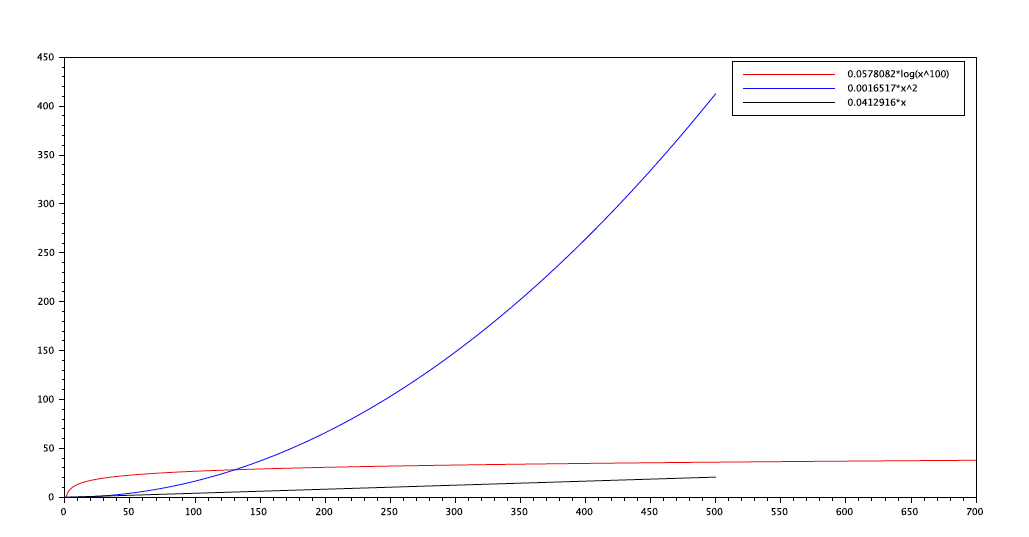
\includegraphics[width=0.9\linewidth]{imagenes/funciones}
\caption{Funciones de coste de cada calentador del modelo mejorado}
\label{fig:funciones}
\end{figure}

\section{Conclusiones}

En este caso práctico, hemos visto cómo utilizar Scilab para resolver un problema de programación no lineal.

\clearpage

\section{Código Scilab utilizado}

A continuación se muestra el código Scilab realizado para la resolución de las cuestiones de evaluación planteadas:

\verbatiminput{programa-scilab/coste.sce}
\end{document}